% IFN680 Project 3 technical report.
% Generated by tools/build_report.py. Every number below is printed by notebook/main_report.ipynb.
% Build:  tectonic project3_report.tex
\documentclass[10pt,a4paper,twocolumn]{article}

\usepackage[margin=1.5cm,top=0.9cm,bottom=0.8cm]{geometry}
\usepackage{lmodern}
\usepackage[T1]{fontenc}
\usepackage[utf8]{inputenc}
\usepackage{microtype}
\usepackage{graphicx}
\usepackage{booktabs}
\usepackage[font=small,labelfont=bf,skip=3pt]{caption}
\usepackage{titlesec}

\titlespacing*{\section}{0pt}{4pt}{0.5pt}
\titleformat{\section}{\normalfont\bfseries}{\thesection.}{0.5em}{}
\setlength{\parskip}{0pt}
\setlength{\parindent}{1em}
\setlength{\columnsep}{0.6cm}
\setlength{\textfloatsep}{3pt}
\setlength{\intextsep}{3pt}
\setlength{\floatsep}{3pt plus 1pt minus 1pt}
\setlength{\tabcolsep}{4pt}
\pagestyle{empty}

\renewcommand{\topfraction}{0.94}
\renewcommand{\bottomfraction}{0.55}
\renewcommand{\textfraction}{0.06}
\renewcommand{\floatpagefraction}{0.75}

\begin{document}

% Figure 1 is set inside the \twocolumn optional argument rather than as a figure* float. In the
% article class \twocolumn[...] claims the page's double column top region, so a figure* declared
% afterwards can never be placed on page 1 and is silently deferred to page 2.
\twocolumn[{%
\begin{center}
{\large\bfseries Project 3: Aircraft Classification with a Pretrained ResNet-18}\\[2pt]
{\bfseries Group 4}
\end{center}
\vspace{-2pt}
Student 1: Karan Rooprai \hfill Student 1 ID: n12498122 \\
Student 2: Nhu Hieu Nguyen \hfill Student 2 ID: n12194778 \\
\vspace{2pt}

\begin{center}
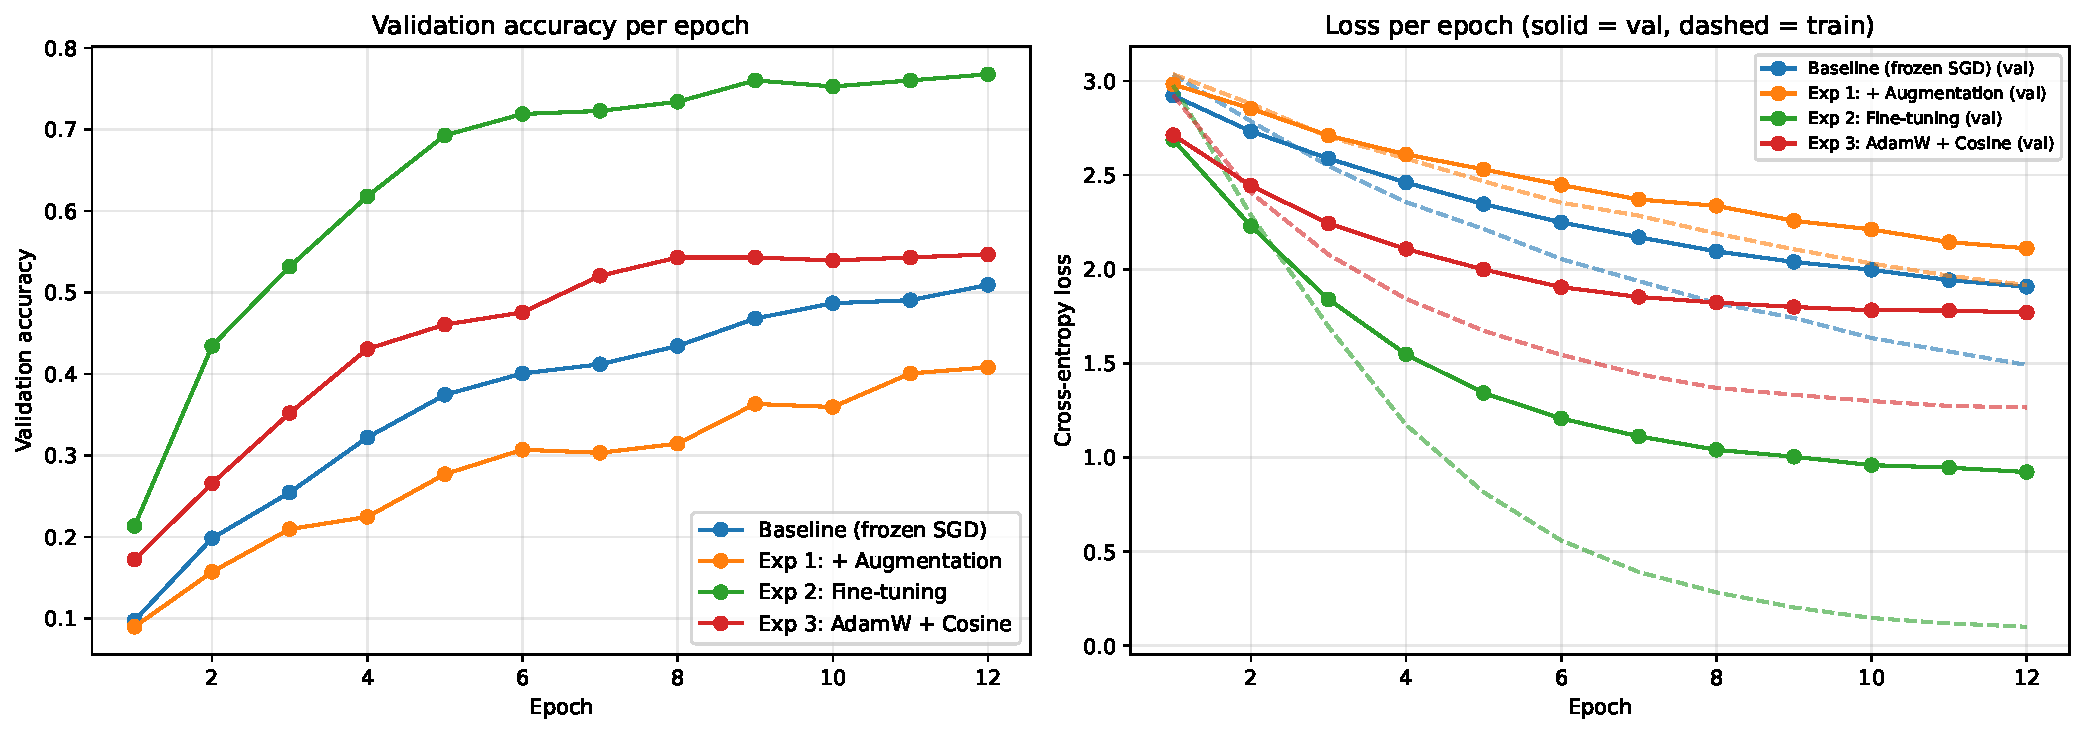
\includegraphics[width=0.88\textwidth]{figures/learning_curves.pdf}
\end{center}
\vspace{-8pt}
\begin{quote}
\small\textbf{Figure 1.} Validation accuracy (left) and cross-entropy loss (right) per epoch for
the baseline and all three experiments, on shared axes. Dashed lines on the right are training
loss. Fine-tuning (green) separates from the three frozen-backbone runs within two epochs.
\end{quote}
\vspace{4pt}
}]

A pretrained ResNet-18 (ImageNet weights) was adapted by transfer learning to classify the
20-class FGVC-Aircraft subset. The \texttt{trainval} folder of 1,331 images was
divided by a stratified 1,064/267 split into training and validation sets; the 669 test
images were held out and used once, for the final evaluation only. Every image was resized to
$224\times224$ and normalised with the ImageNet mean and standard deviation to match the pretrained
backbone, and the 1000-way ImageNet head was replaced with a fresh 20-way linear layer.
The three experiments follow a controlled design: each alters a single variable relative to a
common baseline and trains for 12 epochs, so any change in validation accuracy is
attributable to that one factor.

\section{Baseline model}
The baseline uses ResNet-18 as a fixed feature extractor: the convolutional backbone is frozen and
only the new classification head is trained, with plain SGD (learning rate 0.001, momentum 0.9) on
un-augmented images. This establishes the performance floor every experiment must beat. It reached
a best validation accuracy of \textbf{0.5094} (Table~1; blue curve, Figure~1). The frozen
ImageNet features separate the twenty aircraft types moderately well, but because the backbone
cannot adapt, the head alone cannot capture the fine-grained differences between visually similar
variants.

\section{Experiment 1: Data augmentation}
\textbf{Hypothesis:} randomly flipping, rotating ($\pm15^\circ$) and colour-jittering the training
images exposes the frozen extractor to more varied views, reducing over-fitting and improving
validation accuracy. \textbf{Result: not supported.} Augmentation lowered best validation accuracy
to 0.4082, a drop of $-$0.1011 below the baseline (orange curve, Figure~1). With the backbone frozen
the network cannot adapt its features to the distorted inputs, so augmentation pushes images into
regions of the fixed ImageNet feature space that the linear head has not learned, and 12
epochs are too few to compensate. Augmentation therefore hurts a pure feature-extraction setup on
this dataset.

\section{Experiment 2: Fine-tuning the backbone}
\textbf{Hypothesis:} ImageNet features are generic, so unfreezing the backbone and letting every
layer adapt to aircraft should capture fine-grained variant differences and lift accuracy well
above the frozen baseline. \textbf{Result: strongly supported.} Unfreezing the backbone was the
only change from the baseline, keeping the identical SGD optimiser and 0.001 learning rate; it
raised best validation accuracy to \textbf{0.7678}, a gain of +0.2584 (green curve, Figure~1). This is
by far the largest single improvement, confirming that adapting the convolutional features, and
not just the classifier, is what fine-grained aircraft recognition requires.

\section{Experiment 3: AdamW and cosine annealing}
\textbf{Hypothesis:} replacing plain SGD with AdamW (adaptive updates with decoupled weight decay)
and decaying the learning rate on a cosine schedule should give faster, more stable convergence of
the frozen head and a modest accuracy gain. \textbf{Result: supported, modestly.} With the backbone
frozen and images un-augmented, best validation accuracy rose to 0.5468, a gain of +0.0375 over
the baseline (red curve, Figure~1). AdamW converges faster and to a slightly better optimum than
SGD, but with the backbone still frozen the ceiling is low, so the gain is real but small beside
fine-tuning.

Optimiser, decoupled weight decay and schedule are varied together as one variable: the
optimisation strategy, the axis the task description names. They are not separable the way a single
hyperparameter is: decoupled weight decay is the very thing that distinguishes AdamW from Adam, and
AdamW under cosine annealing is a different procedure rather than another setting of the same one.
Everything outside that axis
(frozen backbone, un-augmented data, 12 epochs, batch size, 0.001 base learning rate)
is identical to the baseline, so the comparison stays controlled.

\begin{table}[t]
\centering
\small
\begin{tabular}{lrr}
\toprule
Model & Best val.\ acc. & $\Delta$ base \\
\midrule
Baseline (frozen, SGD)     & 0.5094 & n/a \\
Exp 1: + Augmentation      & 0.4082      & $-$0.1011 \\
Exp 2: Fine-tuning         & 0.7678       & +0.2584 \\
Exp 3: AdamW + cosine      & 0.5468    & +0.0375 \\
\bottomrule
\end{tabular}
\caption{Best validation accuracy of the baseline and each single-variable experiment.}
\end{table}

% Declared here, well before the text that discusses it, because a figure* can only be placed at
% the top of a page at or after its declaration point. Declared at the end of the document it has
% no page top left to claim and LaTeX defers it to a float page of its own -- a third page, which
% is a zero for the report. Figure 1 is hand-set inside \twocolumn[...] and is not a float, so the
% float counter has to be advanced by hand or this caption also prints as "Figure 1".
\setcounter{figure}{1}
\begin{figure*}[t]
\centering
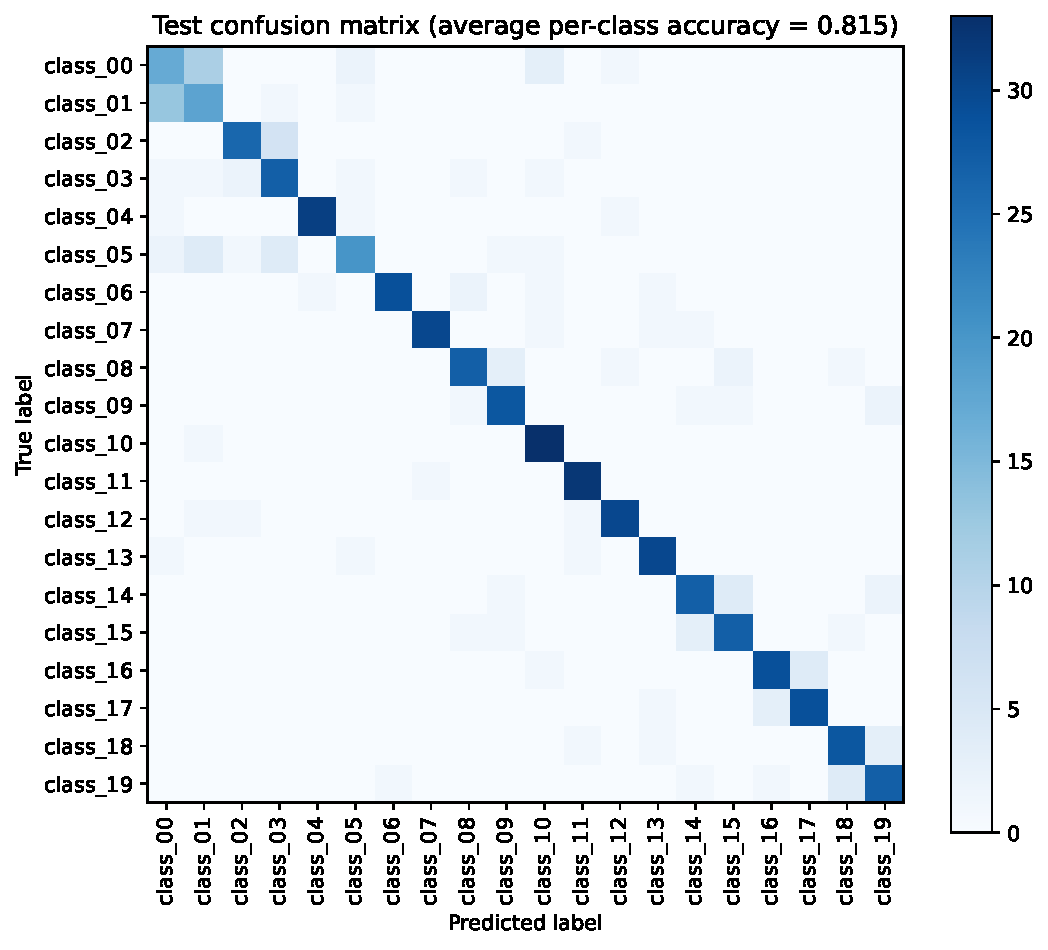
\includegraphics[width=0.44\textwidth]{figures/confusion_matrix.pdf}
\caption{Confusion matrix of the final model on the 669 test images, shown as a heatmap;
rows are true classes, columns predicted. The off-diagonal counts quoted in the text are printed
by \texttt{main\_report.ipynb} rather than read from this figure.}
\end{figure*}

\section{Best model}
\textbf{Rationale.} The final model keeps only the changes that improved validation accuracy over
the baseline. Fine-tuning (+0.2584) and AdamW with cosine annealing (+0.0375) both helped and are
retained; augmentation is excluded, because it reduced accuracy and so is not a winning
ingredient. The final model is therefore an unfrozen ResNet-18 trained with AdamW and cosine
annealing on un-augmented images. It was chosen on best mean validation accuracy rather than on
stability or hardest-class performance, because the margin between fine-tuning and every
alternative (+0.2584) is far larger than the epoch-to-epoch variation visible in Figure~1.

Combining two separately validated changes alters the optimisation problem, so the learning rate
was cut to 0.0001 for the final run: AdamW's adaptive steps on every backbone layer at 0.001 are
more aggressive than either experiment tested, since Experiment~2 used SGD on all layers and
Experiment~3 used AdamW on the head alone. This is the one deliberate departure from a validated
configuration, and it is a design judgement rather than a measured result: once the model is
refit on all of \texttt{trainval}, no validation data survives on which to tune it.

\textbf{Result.} \textbf{The final model was retrained on the entire \texttt{trainval} set (all
1,331 images, training plus validation, no validation split) for 15 epochs, and
every figure reported here is measured on the 669 held-out test images with that refit model,
evaluated once.} It achieves an average per-class accuracy of \textbf{0.8148}, comfortably
exceeding the required 0.75, with overall accuracy 0.8146 and a macro-averaged F1 of 0.8152.
Average per-class accuracy, the mean of the 20 per-class recall values, is the
reported metric rather than overall accuracy because it weights every aircraft type equally
instead of letting the larger or easier classes dominate. The two agree closely here only because
the test split is balanced. Macro F1 is given alongside because recall alone cannot see a class
the model over-predicts. The test confusion matrix is Figure~2.

\section{Potential and limitations}
The strong diagonal in Figure~2 shows most classes are recognised reliably: 7 of
20 score above 0.87 and the best (class\_10, class\_11) reach 0.971 and 0.970. The
clear weakness is class\_00 at 0.500, which is confused with class\_01 in both directions:
13 class\_01 images are predicted as class\_00 and 11 the other way, indicating two
visually near-identical variants the model cannot separate. class\_05 (0.606) and class\_02
(0.788) fail similarly against look-alike types. The fine-tuned model also reaches
1.00 training accuracy within a few epochs, so the gap of roughly 0.19 to test performance
reflects real over-fitting, which the small per-class support makes hard to avoid: at roughly
669$/$20 test images per class, a single extra error moves a class score by about
three points.

For the target application the method is promising: 0.8148 average per-class accuracy over twenty
types, from barely a thousand labelled images and a backbone that trains in minutes, shows transfer
learning suits a catalogue task with narrow visual differences. The anticipated limitations are the
near-identical variants above, unlikely to separate without finer-grained supervision or
higher-resolution inputs; the small per-class support, which makes every class score coarse; and
uncalibrated output scores, which should not be read as probabilities in deployment. The obvious
next steps are reintroducing light augmentation now the backbone is trainable (augmentation
regularises a fine-tuned network differently from a frozen one, so Experiment~1 does not settle the
question), tuning weight decay or dropout, early stopping, and a deeper backbone such as
ResNet-34 for the hardest look-alike pairs.

\end{document}
